\documentclass[13pt]{article}
 \usepackage{fontspec}
 \usepackage[english]{babel} 
 \newfontfamily\skt[Script=Devanagari]{Siddhanta}
 \usepackage{parskip}
 \usepackage[dvipsnames]{xcolor}
 \usepackage{graphicx}
\graphicspath{ {images/} }
\usepackage{float}
\usepackage{wrapfig}
\usepackage{array}
\title{\textbf{A simple protocol for the worship of the god Kumāra}}
\author{}
\date{}

\begin{document}
\maketitle
\begin{center}
{\skt
देव-देवं नमस्यामि कुमारं वरमच्युतम् ।\\
कार्त्तिकेयं दुराराध्यं वह्नि-तेजः समुद्भवम् ।। 
}\\
 \end{center}
\section{{\skt मन्त्राणि}}
\subsection{{\skt ध्यानम् }}
{\skt ॐ सिन्दुरारुण-कान्तिम् इन्दु-वदनं केयूर-हारादिभिर् \\
दिव्यैराभरणैर् विभूषित तनुं स्वर्गस्य सौख्य प्रदम् ।\\ 
अम्भोजाभय शक्ति कुक्कुटधरं रक्ताङ्ग रागांशुकं \\
सुब्रह्मण्यम् उपास्महे प्रणमतां भीतिप्रणाशोद्यतम् ॥
}\\[8pt]
Om. He is of vermilion color and his face is beautiful as the moon; his body is adorned with beautiful armlets, garlands, and shining ornaments and he provides heavenly joy. His hands hold a lotus, the abhaya-mudrā, the spear and the cock banner; he is raimented in red, anointed with red unguent and he destroys the fears of his worshipers.
\subsection{{\skt मूलमण्त्राणि }}
{\normalsize{\skt ॐ कं क्षं कं कार्त्तिकेयाय फट् ॥\\
ॐ श्रीं ह्रीं क्लीम् ऐं सौं शरवनभवाय नमः ॥\\
ॐ वचद्भुवे नमः ॥\\
ॐ भुवे नमः स्वाहा ॥\\
ॐ षं षण्मुखाय नमः ॥\\
ॐ श्रीम् ए इ उ न श्रीं रीं कुमाराय नमः ॥
}\\
\subsection{{\skt गायत्री }}
{\skt ॐ तत्-कुमाराय विद्महे कार्त्तिकेयाय धीमहि । तन्नः स्कन्दः प्रचोदयात् ॥
}\\[8pt]
May we know of that Kumāra, [hence] we focus upon Kārttikeya. May that Skanda impel us.
\subsection{{\skt कुमार-वन्दनम् }}
{\skt ॐ जयन्ताय नमः । ॐ अग्निवेश्याय नमः । ॐ कृत्तिकापुत्राय नमः । ॐ भुतपतये नमः । ॐ सेनान्ये नमः । ॐ गुहाय नमः । ॐ हेमशूलय नमः । ॐ विशालाक्षाय नमः ॥
}
\subsection{{\skt षष्ठी-वन्दनम् }}
{\skt ॐ षष्ठ्यै नमः । ॐ देवसेनायै नमः । ॐ बिडालवहनायै नमः । ॐ कौमार्यै नमः । ॐ विशाखायै नमः । ॐ षण्मुखायै नमः ॥  
}
\subsection{{\skt अस्त्र-सहित-सर्व-देव-वन्दनम् }}
{\skt ॐ स्कन्दाय ब्रह्मण्याय देवसेनापतये मेरुर्-इवाचलाय शक्ति-हस्ताय नमः । ॐ शक्राय त्रिदशनां महेश्वराय पाण्डूर-गज-वाहनाय वज्र-हस्ताय नमः । ॐ विष्णवे वासुदेवाय दानव-सुदनाय चक्र-हस्ताय नमः । ॐ अग्नये हुताशनाय शक्ति-पाणये नमः । ॐ यमाय राजाय काल-दण्ड-हस्ताय नमः । ॐ वरुणाय धर्मराजाय पाश-विचक्र-धराय नमः । ॐ वैश्रवणाय धनेश्वराय शिबिका-धरय नमः । ॐ निरृताय यातुराजाय खद्ग-शक्तिधराय नमः । ॐ वायवे समीरणाय अङ्कुश-हस्ताय नमः । ॐ अश्विभ्यां दीप्यामानौषधि-गृहितृभ्यां नमः । ॐ धात्रे धनुर्-हस्ताय  नमः । ॐ जयाय मुसल-हस्ताय  नमः । ॐ त्वष्ट्रे महाबलाय पर्वत-धराय नमः । ॐ अंशाय शक्ति-धराय  नमः । ॐ मृत्यु-देवाय परशु-हस्ताय  नमः । ॐ रुद्राय महादेवाय पिनाक-पाशुपत-धराय  नमः । ॐ अर्यम्णे घोर-परिघ-गृहीत्रे नमः । ॐ मित्राय क्षुर-नेमि-चक्र-धराय  नमः । ॐ पुष्णे चक्र-पाणये  नमः । ॐ भगाय शर-कार्मुक-धराय  नमः । ॐ सवित्रे निस्त्रिंश-हस्ताय नमः । ॐ मरुद्भ्यश् चित्रायुधेभ्यो  नमः ॥ 
}
\subsection{{\skt कृत्तिका-वन्दनम् }}
{\skt ॐ अम्बा दुला नितत्नी अभ्रयन्ती मेघयन्ती वर्षयन्ती छुपुणिका कुमार-मातृभ्यो नमो नमः ॥
}
\subsection{{\skt मातृ-वन्दनम् }}
{\skt ॐ आवेशिनी ह्य् अश्रुमुखी कुतुहली हस्तिनी जृंभिणी स्तंभिनी मोहिनी च । कृष्णा विशाखा विमला ब्रह्मरात्री भ्रातृव्य-संघेषु पतन्त्य् अमोघास् ताभ्यो वै मातृभ्यो नमो नमः ॥ 
}
\subsection{{\skt तर्पणम् }}
{\skt सनत्कुमारं तर्पयामि । स्कन्दं तर्पयामि । इन्द्रं तर्पयामि । षष्ठीं तर्पयामि । षण्मुखं तर्पयामि । जयन्तं तर्पयामि । विशाखं तर्पयामि । महासेनं तर्पयामि । सुब्रह्मण्यं तर्पयामि । स्कन्दपार्षदांस् तर्पयामि । स्कन्दपार्षदीश्च तर्पयामि ।
 }
\subsection{{\skt तर्पणम् }}
\subsection{{\skt बलिहरणम् }}
{\skt आयातु देवो मम कार्त्तिकेयो ब्रह्मण्यपित्रैः सह मातृभिश् च ।\\
भ्रात्रा विशाखेन च विश्वरूप इमम् बलिं सानुचर जुषस्व ॥ 
}\\[8pt]
May the god Kārttikeya, come with his fathers and mothers.\\
Along with his brother Viśākha, multi-formed, may he with his followers be pleased with this bali of mine.
\subsection{{\skt प्रार्थना }}
{\skt  देवम् प्रपद्ये वरदम् प्रपद्ये स्कन्दम् प्रपद्ये च कुमारम् उग्रम् ।\\
षण्णां सुतं कृत्तिकानां षडास्यम् अग्नेः पुत्रं महासेनम् प्रपद्ये ॥
}\\[8pt]
I take refuge in the god, the boon-giver, Skanda , the fierce Kumāra.\\
I take refuge in the son of the six Kṛttikā-s, the six-faced one, the son of Agni, [who is] Mahāsena
\section{Vidhi}
\begin{enumerate}
\item The rite may be done on a ṣaṣṭhī day or daily.
\item Meditate on Kumāra either mentally or using an idol or the yantra (see below) with the dhyānam till you are able to form a mental image of the deity.
\item  Then perform japa with one or each of the 6 mūla-mantra-s . If using all six, minimally mutter each mantra 6 $\times$. If using just one, do a japa of 108 $\times$ or 1008 $\times$, as per you capacity. You may keep the count with an akṣamālā with rudrākṣa or sphaṭika beads or with the nodes of your fingers. If you are doing a long japa then you may mark every 10 or 100 with a blade of darbha.
\item  Thereafter offer arghya with the gāyatrī either with your cupped palms or with a śaṅkha
\item Then do the vandanam with either flowers, grains or a spoon of water offered with a darvi at each namaḥ. Preferred flowers are kadamba or arka. Kadamba leaves may also be used. Preferred grains are rice or barley.
\item Then offer plain or scented water for tarpaṇa with the darvi. Ghee, tila oil or water mixed with white tila may also be offered.
\item Offer bali at the end. It might be in the form of plain rice, rice mixed with white tila, or  apūpa or maṇḍaka.
\item During the recitation of the prārthanā one may tie a black thread around the wrist of a recipient on behalf of whom you are doing the rite as a rakṣa.
\end{enumerate} 
\section{Yantra}
\begin{figure}[h]
  \centering
    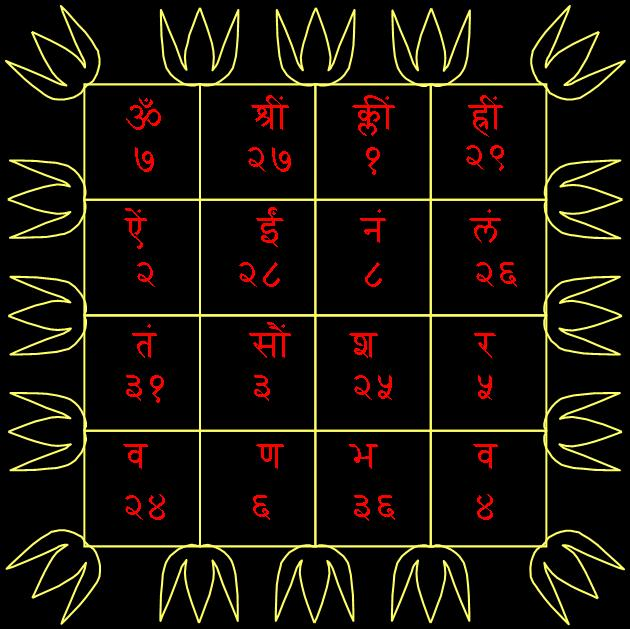
\includegraphics[width=0.5\textwidth]{kaumara_magic_square}
    \caption{The magic square Kaumāra-yantra}
    \label{fig:fig1}
    \end{figure}
    
While during the dhyana and the japa one may focus on one of the below yantra-s (Figure \ref{fig:fig1} or Figure \ref{fig:fig2}). He may inscribe it on copper, silver or gold or draw it repeatedly on a black stone slab or on a wooden board of bamboo for each performance.

\begin{figure}[h]
  \centering
    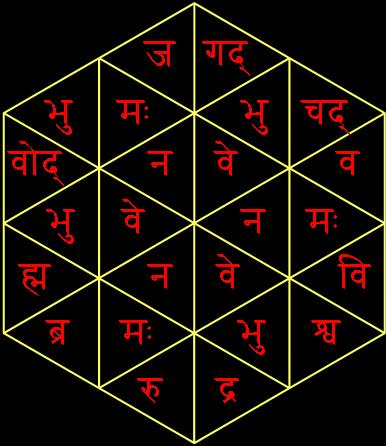
\includegraphics[width=0.5\textwidth]{shaktyuta_mUrti_yantra}
    \caption{The hexagonal Kaumāra-yantra}
    \label{fig:fig2}
    \end{figure}
\end{document}